\ifx\wholebook\relax \else
% ------------------------

\documentclass[b5paper]{ctexart}
\usepackage[nomarginpar
  %, margin=.5in
]{geometry}

\addtolength{\oddsidemargin}{-0.05in}
\addtolength{\evensidemargin}{-0.05in}
\addtolength{\textwidth}{0.1in}

\usepackage[cn]{../../../prelude}

\setcounter{page}{1}

\begin{document}

\title{红黑树}

\author{刘新宇
\thanks{{\bfseries 刘新宇} \newline
  Email: liuxinyu95@gmail.com \newline}
  }

\maketitle
\fi

\markboth{红黑树}{基本算法}

\ifx\wholebook\relax
\chapter{红黑树}
\numberwithin{Exercise}{chapter}
\fi

% ================================================================
%                 Introduction
% ================================================================
在第二章的例子中,我们使用二叉搜索树来统计文章中每个词的出现次数。一个自然的想法是用二叉搜索树处理通讯录,用来查询联系人的电话。如下面的例子代码所示:

\lstset{frame = single}
\begin{lstlisting}[language=Bourbaki]
void addrBook(Input in) {
    bst<string, string> dict
    while (string name, string addr) = read(in)) {
        dict[name] = addr
    }
    loop {
        string name = read(console)
        var addr = dict[name]
        if (addr == null) {
            print("not found")
        } else {
            print("address: ", addr)
        }
    }
}
\end{lstlisting}

但这个方法的性能不佳,尤其是搜索诸如Zara、Zed、Zulu等姓名时更加明显。通讯录通常是按照字典顺序排列的。如果依次把自然数1, 2, 3, ..., $n$插入二叉搜索树,就会得如图\ref{fig:unbalanced-tree}中的结果。这是一棵极不平衡的二叉树。对于高为$h$的二叉搜索树,$lookup()$的复杂度为$O(h)$。如果树比较平衡,我们就能够达到$O(\lg n)$的性能。但在这一极端情况下,查找的性能退化为$O(n)$。几乎等同于列表扫描。


\begin{figure}[htbp]
    \centering
	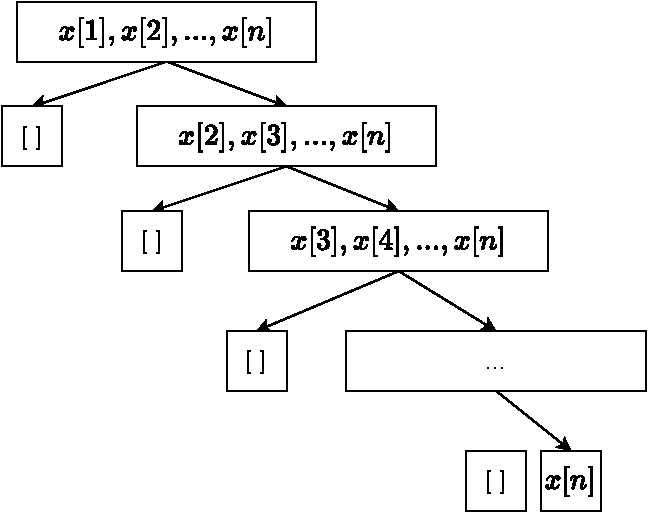
\includegraphics[scale=0.5]{img/unbalanced.ps}
    \caption{不平衡的树} \label{fig:unbalanced-tree}
\end{figure}


\begin{Exercise}
\Question{对于较大的通讯录,为了加快构建速度,有人使用两个并发的任务。一个任务从头部向后,另外一个任务从后向前读取。当两个任务在中间相遇时结束。这样构建出的二叉搜索树是什么样子的?如果把通讯录分成更多片断,使用更多的任务会得到什么结果?}
\Question{参考图\ref{fig:unbalanced-trees},找出更多的不平衡情况。}
\end{Exercise}

\begin{figure}[htbp]
  \centering
  \subcaptionbox{}{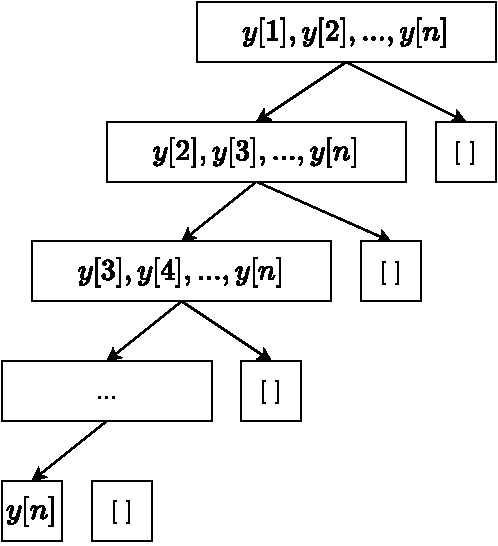
\includegraphics[scale=0.4]{img/unbalanced-2.ps}}
  \subcaptionbox{}{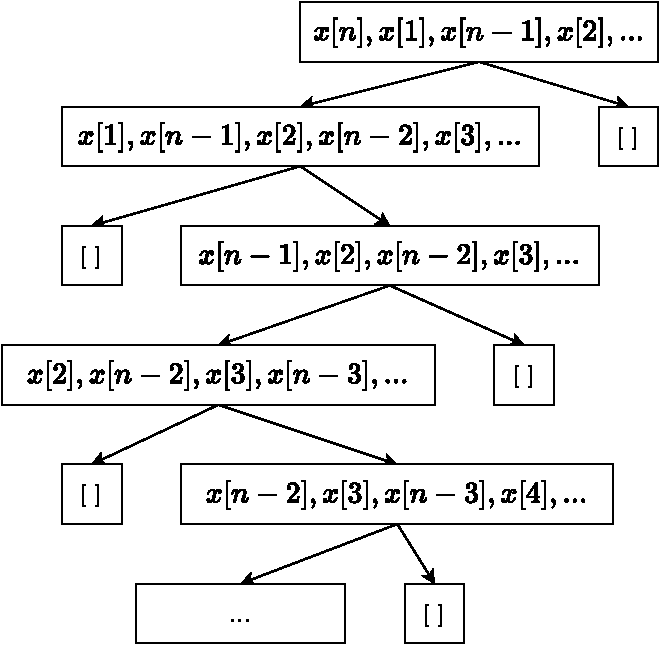
\includegraphics[scale=0.4]{img/unbalanced-zigzag.ps}} \\
  \subcaptionbox{}{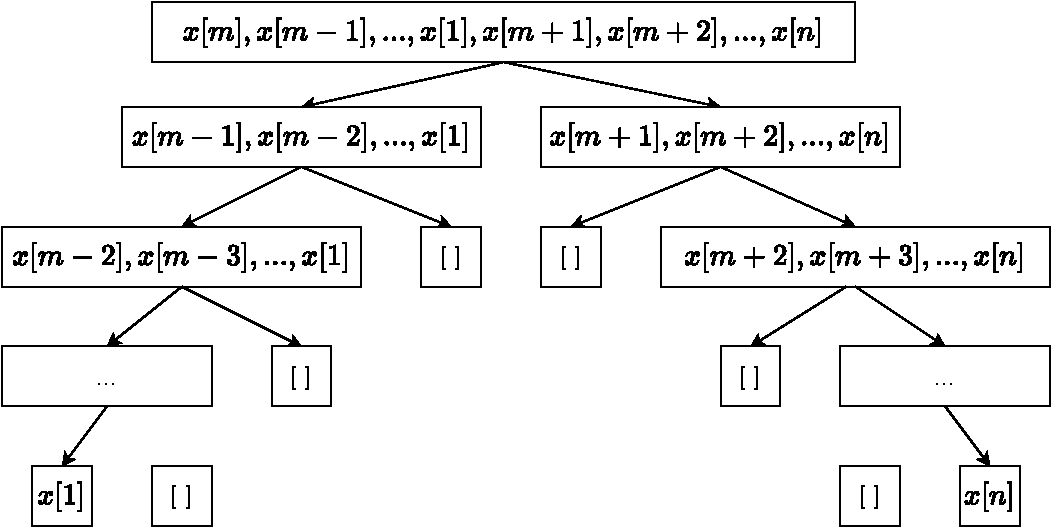
\includegraphics[scale=0.4]{img/unbalanced-3.ps}}
  \caption{一些不平衡的二叉树}
  \label{fig:unbalanced-trees}
\end{figure}

\subsection{平衡}

为了避免这种极不平衡的情况,我们可以将输入序列打乱(\cite{CLRS}第12.4节)。但这种方法有一定的局限性,如果序列是用户交互输入的,则无法应用这一方法。人们找到了一些解决平衡性的方法,它们大多依赖于二叉树的旋转操作。旋转操作可以在改变树结构的同时,保持元素间顺序不变。这一章介绍红黑树。它是一种被广泛使用的自平衡二叉搜索树。下一章我们介绍另外一种自平衡树――AVL树。第8章还会介绍伸展树,它能够随着操作,逐步把树变得平衡。

\subsection{树旋转}
\index{树旋转}

\begin{figure}[htbp]
  \centering
  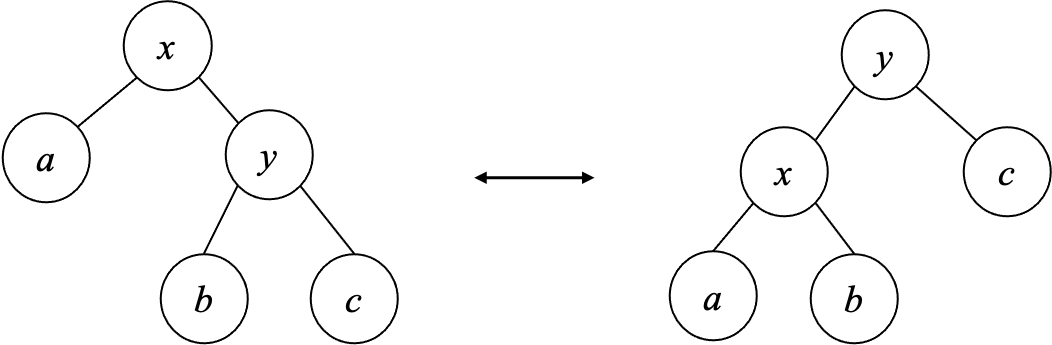
\includegraphics[scale=0.4]{img/tree-rotation.png}
  \caption{树的左右旋转}
  \label{fig:tree-rotation}
\end{figure}

树旋转在保持中序遍历结果不变的情况下,改变树的结构。存在多个不同的二叉树对应到一个特定的中序遍历顺序。图\ref{fig:tree-rotation}描述了旋转操作。

旋转操作可以通过模式匹配来定义:

\be
\begin{array}{rcl}
rotate_l\ ((a, x, b), y, c) & = & (a, x, (b, y, c)) \\
rotate_l\ T & = & T \\
\end{array}
\ee

和

\be
\begin{array}{rcl}
rotate_r\ (a, x, (b, y, c)) & = & ((a, x, b), y, c)) \\
rotate_r\ T & = & T \\
\end{array}
\ee

如果模式没有匹配(例如两棵子树都为空),每个式子的第二行保证树不变。旋转操作也可以通过一系列步骤实现。我们需要将子树和父引用设置正确。在旋转时,我们传入根节点$T$和要旋转的子树$x$:

\begin{algorithmic}[1]
\Function{Left-Rotate}{$T, x$}
  \State $p \gets$ \Call{Parent}{$x$}
  \State $y \gets$ \Call{Right}{$x$} \Comment{设$y \ne$ NIL}
  \State $a \gets$ \Call{Left}{$x$}
  \State $b \gets$ \Call{Left}{$y$}
  \State $c \gets$ \Call{Right}{$y$}
  \State \Call{Replace}{$x, y$}  \Comment{用$y$替换$x$}
  \State \Call{Set-Subtrees}{$x, a, b$} \Comment{令$a, b$为$x$的子树}
  \State \Call{Set-Subtrees}{$y, x, c$} \Comment{令$x, c$为$y$的子树}
  \If{$p = $ NIL}  \Comment{此前$x$是根节点}
    \State $T \gets y$
  \EndIf
  \State \Return $T$
\EndFunction
\end{algorithmic}

右旋\textproc{Right-Rotate}的实现是对称的,我们将其留作练习。\textproc{Replace}($x$, $y$)使用$y$替换$x$:

\begin{algorithmic}[1]
\Function{Replace}{$x, y$}
  \State $p \gets$ \Call{Parent}{$x$}
  \If{$p$ = NIL} \Comment{$x$是根节点}
    \If{$y \ne$ NIL}
           \Call{Parent}{$y$} $\gets$ NIL
    \EndIf
  \ElsIf{\Call{Left}{$p$} $= x$}
    \State \Call{Set-Left}{$p$, $y$}
  \Else
    \State \Call{Set-Right}{$p$, $y$}
  \EndIf
  \State \Call{Parent}{$x$} $\gets$ NIL
\EndFunction
\end{algorithmic}

\textproc{Set-Subtrees}($x, L, R$)将$L$设为$x$的左子树,$R$设为右子树:

\begin{algorithmic}[1]
\Function{Set-Subtrees}{$x, L, R$}
  \State \Call{Set-Left}{$x, L$}
  \State \Call{Set-Right}{$x, R$}
\EndFunction
\end{algorithmic}

它进一步调用\textproc{Set-Left}和\textproc{Set-Right}完成子树的设置:

\begin{algorithmic}[1]
\Function{Set-Left}{$x, y$}
  \State \Call{Left}{$x$} $\gets y$
  \If{$y \ne$ NIL}
    \Call{Parent}{$y$} $\gets x$
  \EndIf
  \EndFunction

\Statex

\Function{Set-Right}{$x, y$}
  \State \Call{Right}{$x$} $\gets y$
  \If{$y \ne$ NIL}
    \Call{Parent}{$y$} $\gets x$
  \EndIf
\EndFunction
\end{algorithmic}

通过对比,可以看到模式匹配如何简化树旋转的实现。从这一点出发Okasaki在1995年实现了红黑树的纯函数式算法\cite{okasaki}。

\begin{Exercise}
\Question{实现右旋\textproc{Right-Rotate}操作。}
\end{Exercise}

\section{定义}
\index{红黑树}

红黑树是一种自平衡二叉搜索树\cite{wiki-rbt}。它是2-3-4树的等价形式\footnote{第7章,B树。对于任一2-3-4树,都存在至少一棵红黑树,其元素顺序相同。}。通过对节点进行着色和旋转,红黑树可以高效地地保持平衡性。我们在二叉搜索树的定义上给节点赋予红、黑颜色。我们称一棵树为红黑树,如果它满足下面5条性质\cite{CLRS}:

\index{红黑树!红黑性质}
\begin{enumerate}
\item 节点的颜色为红色或黑色。
\item 根节点为黑色。
\item 所有的叶节点(NIL)为黑色。
\item 如果一个节点为红色,则它的两个子节点都是黑色。
\item 从任一节点出发到所有叶子节点的路径上包含相同数量的黑色节点。
\end{enumerate}

为什么这5条性质能保证红黑树的平衡性呢?关键在于:从根节点出发到达叶节点的所有路径中,最长路径不会超过最短路径两倍。性质4保证了不存在两个连续的红色节点。因此,最短的路径只含有黑色的节点。任何更长的路径一定含有红色节点。根据性质5,从任何节点出发的所有的路径都含有相同数量的黑色节点,自然这条对于根节点也成立。这就最终保证了没有任何路径超过最短路径长度的两倍\cite{wiki-rbt}。图\ref{fig:rbt-example-with-nil}的例子展示了一棵红黑树。

\begin{figure}[htbp]
  \centering
  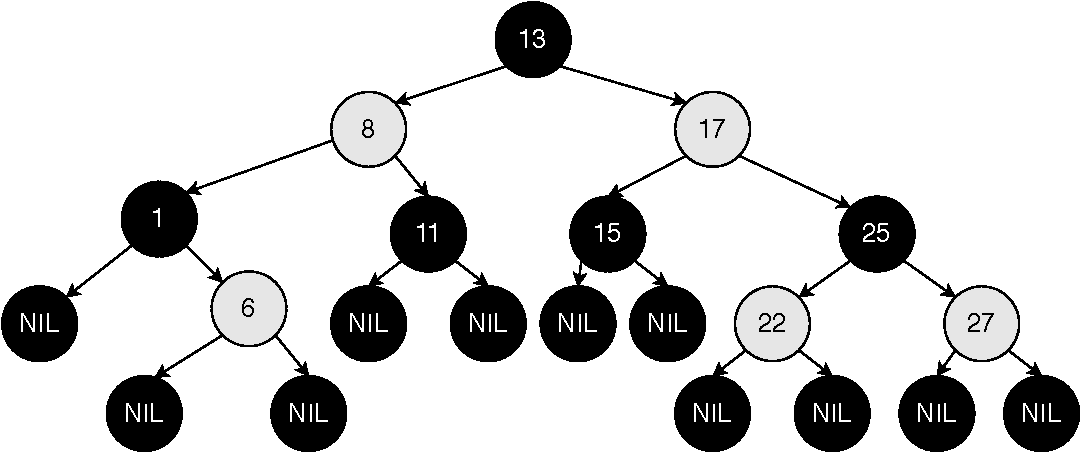
\includegraphics[scale=0.5]{img/rbt-example-with-nil.ps}
  \caption{红黑树}
  \label{fig:rbt-example-with-nil}
\end{figure}

由于所有的NIL节点都是黑色的,我们通常将NIL节点隐藏不画出,如图\ref{fig:rbt-example-with-nil}所示。所有不改变树结构的操作都和二叉搜索树相同,包括查找、最大、最小值等。只有插入和删除操作是特殊的。

\begin{figure}[htbp]
  \centering
  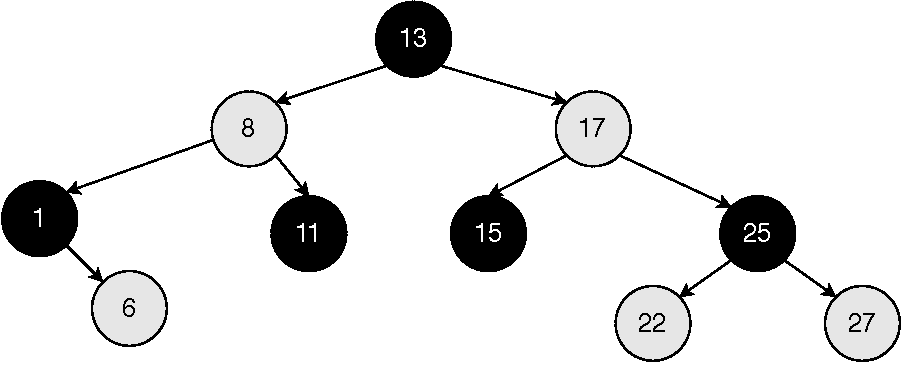
\includegraphics[scale=0.5]{img/rbt-example.ps}
  \caption{隐藏NIL节点}
  \label{fig:rbt-example}
\end{figure}

下面的例子程序在二叉搜索树的基础上增加了颜色定义:

\begin{Haskell}
data Color = R | B
data RBTree a = Empty
              | Node Color (RBTree a) a (RBTree a)
\end{Haskell}

\begin{Exercise}
\Question{证明含有$n$个节点的红黑树,其高度$h$不会超过$2 \lg (n+1)$。}
\end{Exercise}

\section{插入}
\index{红黑树!插入}

插入算法包含两个步骤。第一步和二叉搜索树相同,树可能会变得不再平衡。第二步修复红黑树的颜色性质。插入时,我们令新节点为红色。只要它不是根节点,除了第四条外的所有性质都可以满足。唯一的问题是可能引入两个相邻的红色节点,共有4种情况需要修复。Okasaki发现它们具有统一的形式\cite{okasaki},如图 \ref{fig:insert-fix}所示。

\begin{figure}[htbp]
  \centering
  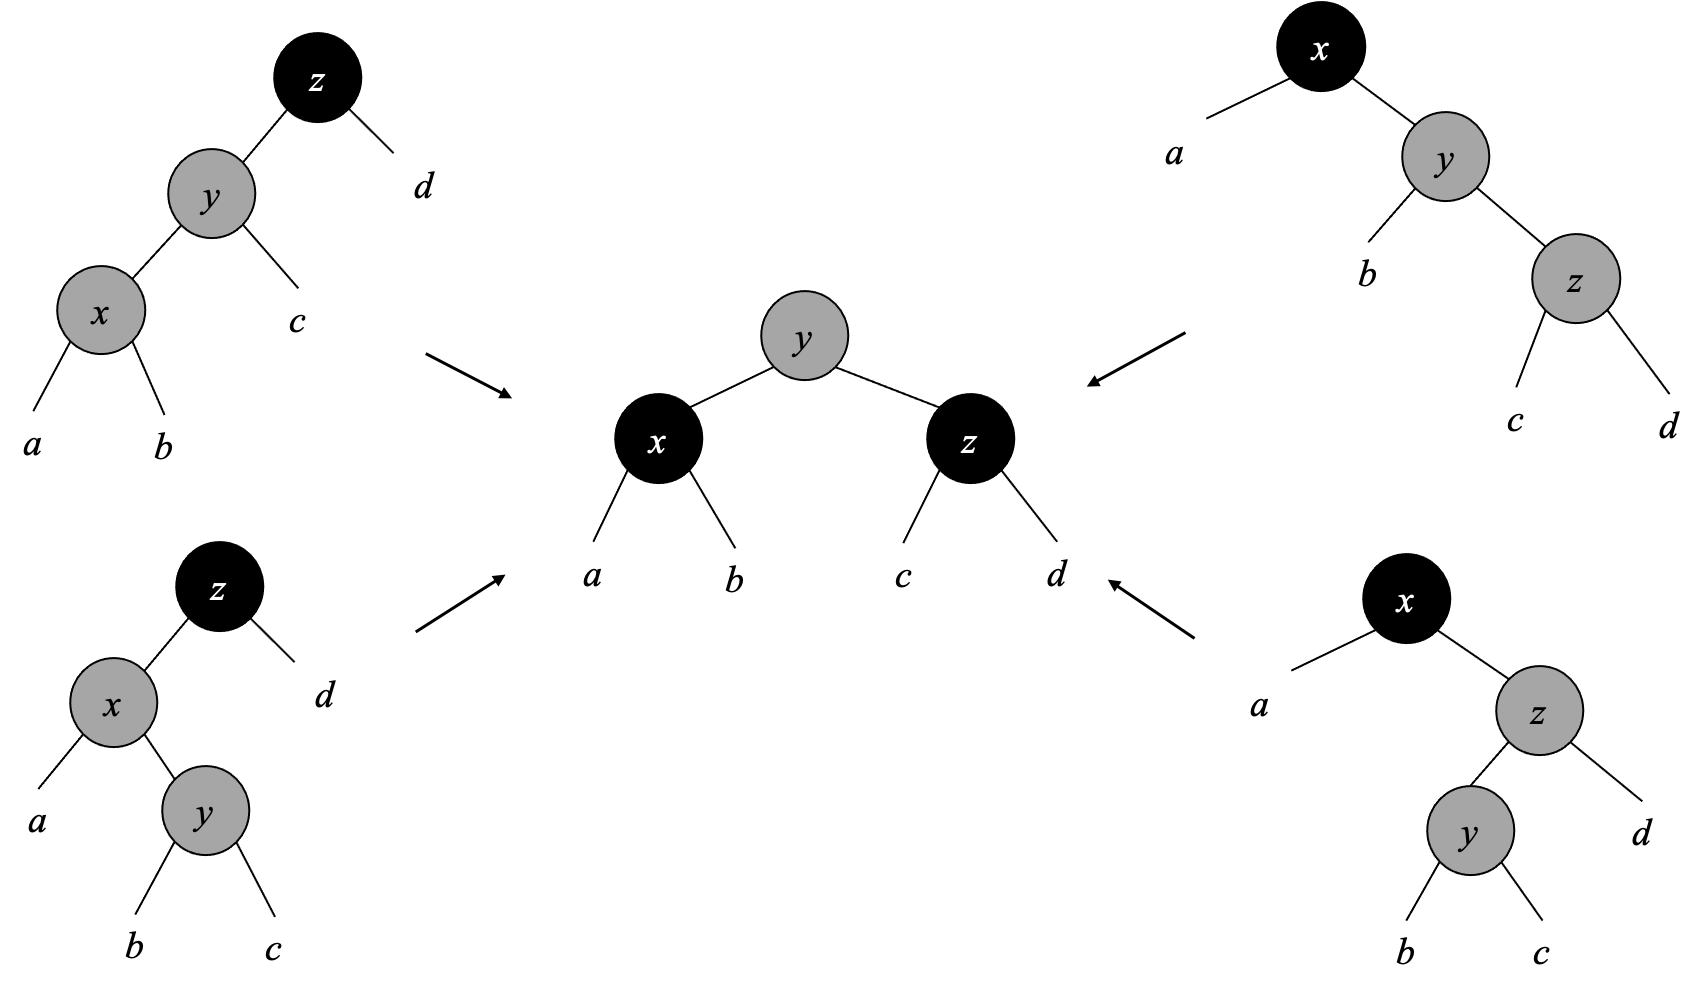
\includegraphics[scale=0.4]{img/insert-fix.png}
  \caption{插入后需要修复的四种情况}
  \label{fig:insert-fix}
\end{figure}

四种情况都把红色向上移动一层。如果进行自底向上的递归修复,最后一步会把根节点染成红色。红黑树性质2要求根节点必须是黑色,因此最后需要把根节点染回黑色。利用模式匹配,我们定义$balance$函数修复平衡性。令节点的颜色变量为$\mathcal{C}$,取值为黑色$\mathcal{B}$或红色$\mathcal{R}$。非空节点表达为一个四元组$T=(\mathcal{C}, l, k, r)$,其中$l$、$r$是左右子树,$k$是值。

\be
\begin{array}{rcl}
%\text{up left:} & & \\
balance\ \mathcal{B}\ (\mathcal{R}, (\mathcal{R}, a, x, b), y, c)\ z\ d & = & (\mathcal{R}, (\mathcal{B}, a, x, b), y, (\mathcal{B}, c, z, d)) \\
%\text{up right:} & & \\
balance\ \mathcal{B}, (\mathcal{R}, a, x, (\mathcal{R}, b, y, c))\ z\ d  & = & (\mathcal{R}, (\mathcal{B}, a, x, b), y, (\mathcal{B}, c, z, d)) \\
%\text{bottom left:} & & \\
balance\ \mathcal{B}\ a\ x\ (\mathcal{R}, b, y, (\mathcal{R}, c, z, d)) & = & (\mathcal{R}, (\mathcal{B}, a, x, b), y, (\mathcal{B}, c, z, d))  \\
%\text{bottom right:} & & \\
balance\ \mathcal{B}\ a\ x\ (\mathcal{R}, (\mathcal{R}, b, y, c), z, d) & = & (\mathcal{R}, (\mathcal{B}, a, x, b), y, (\mathcal{B}, c, z, d))  \\
%\text{otherwise:} & & \\
balance\ T & = & T \\
\end{array}
\ee

如果四种模式都不满足,最后一行保证此时不会改变树的形状。红黑树的插入算法定义如下:

\be
insert\ T\ k = makeBlack\ (ins\ T\ k)
\ee

其中

\be
\begin{array}{rcl}
ins\ \nil\ k & = & (\mathcal{R}, \nil, k, \nil) \\
ins\ (\mathcal{C}, l, k', r)\ k & = & \begin{cases}
  k < k': & balance\ \mathcal{C}\ (ins\ l\ k)\ k'\ r \\
  k > k': & balance\ \mathcal{C}\ l\ k'\ (ins\ r\ k) \\
  \end{cases}
\end{array}
\ee

如果树为空,我们为$k$创建一个红色叶子节点;否则,令树的左右分支和值分别为$l$、$r$、$k'$。比较$k$和$k'$的大小,递归地将$k$插入到子树中。然后用$balance$修复平衡性。最后强制把根节点染成黑色。

\be
makeBlack\ (\mathcal{C}, l, k, r) = (\mathcal{B}, l, k, r)
\ee

下面是对应的例子程序:

\begin{Haskell}
insert t x = makeBlack $ ins t where
    ins Empty = Node R Empty x Empty
    ins (Node color l k r)
        | x < k     = balance color (ins l) k r
        | otherwise = balance color l k (ins r)
    makeBlack(Node _ l k r) = Node B l k r

balance B (Node R (Node R a x b) y c) z d =
                Node R (Node B a x b) y (Node B c z d)
balance B (Node R a x (Node R b y c)) z d =
                Node R (Node B a x b) y (Node B c z d)
balance B a x (Node R b y (Node R c z d)) =
                Node R (Node B a x b) y (Node B c z d)
balance B a x (Node R (Node R b y c) z d) =
                Node R (Node B a x b) y (Node B c z d)
balance color l k r = Node color l k r
\end{Haskell} %$

我们略去了重复值的处理。如果要插入的值已经存在,我们可以覆盖或丢弃,还可以在节点中用一个列表存储相应的数据(\cite{CLRS}, 第269页)。图\ref{fig:insert-example}中给出了两棵红黑树。它们分别由序列11, 2, 14, 1, 7, 5, 8, 4和1, 2, ..., 8构建而成。第二个例子说明,即使序列已序,红黑树仍然保持平衡。

\begin{figure}[htbp]
  \centering
  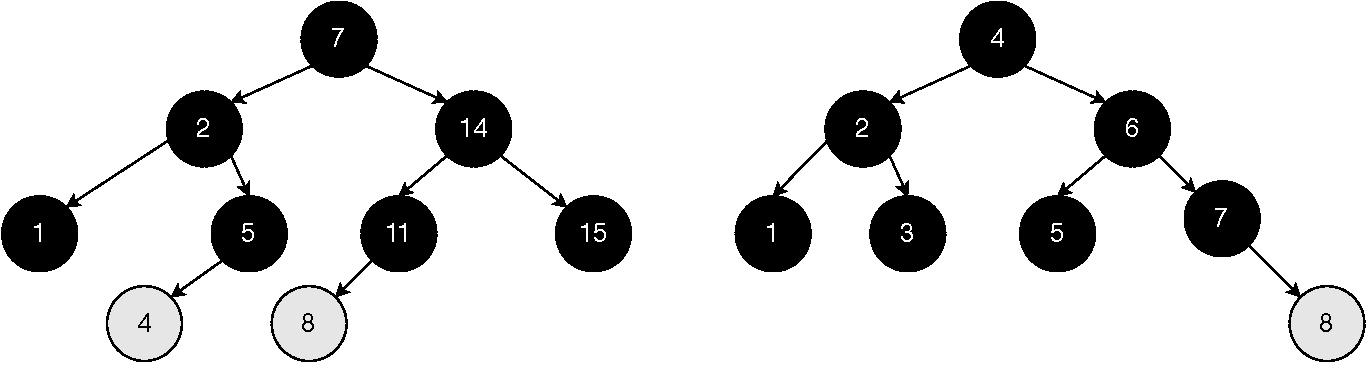
\includegraphics[scale=0.6]{img/insert-haskell.ps}
  \caption{插入产生的红黑树}
  \label{fig:insert-example}
\end{figure}

算法自顶向下递归地进行插入和修复,对于高度为$h$的树,其复杂度为$O(h)$。由于我们始终维护红黑谁的颜色性质,$h$和节点个数$n$呈对数关系。插入算法的复杂度为$O(\lg n)$。

\begin{Exercise}
\Question{不使用模式匹配,同构分别检查四种情况来实现$insert$算法。}
\end{Exercise}

\section{删除}
\index{红黑树!删除}

删除比插入复杂。某些情况下,我们一次性构建一棵只读的树,用于后继的频繁查找\cite{okasaki-blog}。可以通过纯函数式的方法实现红黑树的删除算法\footnote{实际上通过重用不变的部分重新构建了树。这一特性称作persist}。还存在其它一些方法来达到删除的效果。例如,在被删除的节点上加一个标记,当带有删除标记的节点超过50\%的时候,用未标记的节点重建一棵树。删除也会破坏红黑树的性质,因此同样需要进行修复。问题只发生在删除黑色的节点时。这会违反性质5,使得某一路径上的黑色节点数目少于其它的路径。

我们可以通过引入“双重黑色”(\cite{CLRS}第290页)节点来恢复第五条性质。这样的节点算作两个黑色节点。删除黑色节点$x$时,我们将黑色或者向上移动到父节点,或者向下移动到子树上。令接受黑色的节点为$y$。如果$y$原来是红色,将其变为黑色;如果$y$原来是黑色,则变为“双重黑色”,记作$\mathcal{B}^2$。下面的例子程序增加了双重黑色的定义:

\begin{Haskell}
data Color = R | B | BB
data RBTree a = Empty | BBEmpty
              | Node Color (RBTree a) a (RBTree a)
\end{Haskell}

由于所有的空叶子节点都是黑色,当将黑色移动到叶子时,其变为“双重黑色”空节点(\texttt{BBEmpty}或$\pmb{\varnothing}$)。删除时,第一步和普通二叉搜索树相同;如果被删除节点是黑色的,接下来进行修复:

\be
delete = makeBlack \circ del
\ee

这一定义是柯里化的。如果树中只有一个元素,删除后它变为空。为了处理这一情况,我们需要修改$makeBlack$的定义如下:

\be
\begin{array}{rcl}
makeBlack\ \nil & = & \nil \\
makeBlack\ (\mathcal{C}, l, k, r) & = & (\mathcal{B}, l, k, r) \\
\end{array}
\ee

$del$接受一棵树和要删除的元素$k$:

\be
\begin{array}{rcl}
del\ \nil\ k & = & \nil \\
del\ (\mathcal{C}, l, k', r)\ k & = & \begin{cases}
  k < k': & fixB^2(\mathcal{C}, (del\ l\ k), k', r) \\
  k > k': & fixB^2(\mathcal{C}, l, k', (del\ r\ k)) \\
  k = k': & \begin{cases}
    l = \nil: & (\mathcal{C} = \mathcal{B} \mapsto shiftB\ r, r) \\
    r = \nil: & (\mathcal{C} = \mathcal{B} \mapsto shiftB\ l, l) \\
    \text{否则}: & fixB^2(\mathcal{C}, l, k'', (del\ r\ k'')) \\
    & \text{其中}\ k'' = min(r) \\
  \end{cases}
\end{cases}
\end{array}
\ee

如果树为空,结果为$\nil$;否则我们比较$k$和树中的$k'$,如果$k < k'$,我们递归地从左侧分支删除$k$;如果$k > k'$,则递归地从右侧删除。由于递归结果中可能含有双重黑色节点,需要应用$fixB^2$进行修复。当$k = k'$时,我们定位到了要删除的节点。如果任一子树为空,我们用另一子树替换掉当前节点。如果当前节点是黑色的,还需要将黑色移动到子树中。这段定义使用了麦卡锡形式$(p \mapsto a, b)$,它相当于条件表达式:(if $p$ then $a$ else $b$)。如果两棵子树都不为空,我们将右子树中的最小值$k'' = min(r)$切下,并用$k''$替换$k$。

为了保持黑色节点个数,$shiftB$将红色节点变为黑色,将黑色节点变为双重黑色。如果再次应用到双重黑色节点上,则变回黑色。

\be
\begin{array}{rcl}
shiftB\ (\mathcal{B}, l, k, r) & = & (\mathcal{B}^2, l, k, r) \\
shiftB\ (\mathcal{C}, l, k, r) & = & (\mathcal{B}, l, k, r) \\
shiftB\ \nil & = & \pmb{\nil} \\
shiftB\ \pmb{\nil} & = & \nil \\
\end{array}
\ee

下面是相应的例子程序(不包含双重黑色的修复部分):

\begin{Haskell}
delete :: (Ord a) => RBTree a -> a -> RBTree a
delete t k = makeBlack $ del t k where
    del Empty _ = Empty
    del (Node color l k' r) k
        | k < k' = fixDB color (del l k) k' r
        | k > k' = fixDB color l k' (del r k)
        | isEmpty l = if color == B then shiftBlack r else r
        | isEmpty r = if color == B then shiftBlack l else l
        | otherwise = fixDB color l k'' (del r k'') where k''= min r
    makeBlack (Node _ l k r) = Node B l k r
    makeBlack _ = Empty

shiftBlack (Node B l k r) = Node BB l k r
shiftBlack (Node _ l k r) = Node B  l k r
shiftBlack Empty = BBEmpty
shiftBlack BBEmpty = Empty
\end{Haskell}

函数$fixB^2$通过旋转操作和重新染色消除双重黑色。双重黑色节点既可能是分枝节点,也可能是空节点$\pmb{\varnothing}$。有三种情况:

\textbf{情况1:双重黑色的兄弟节点为黑色,并且该兄弟节点有一个红色子节点。}可以通过旋转修复这种情况。共有四种子情况,全部可以变换到一种统一形式。如图\ref{fig:del-case1}所示。

\begin{figure}[htbp]
   \centering
   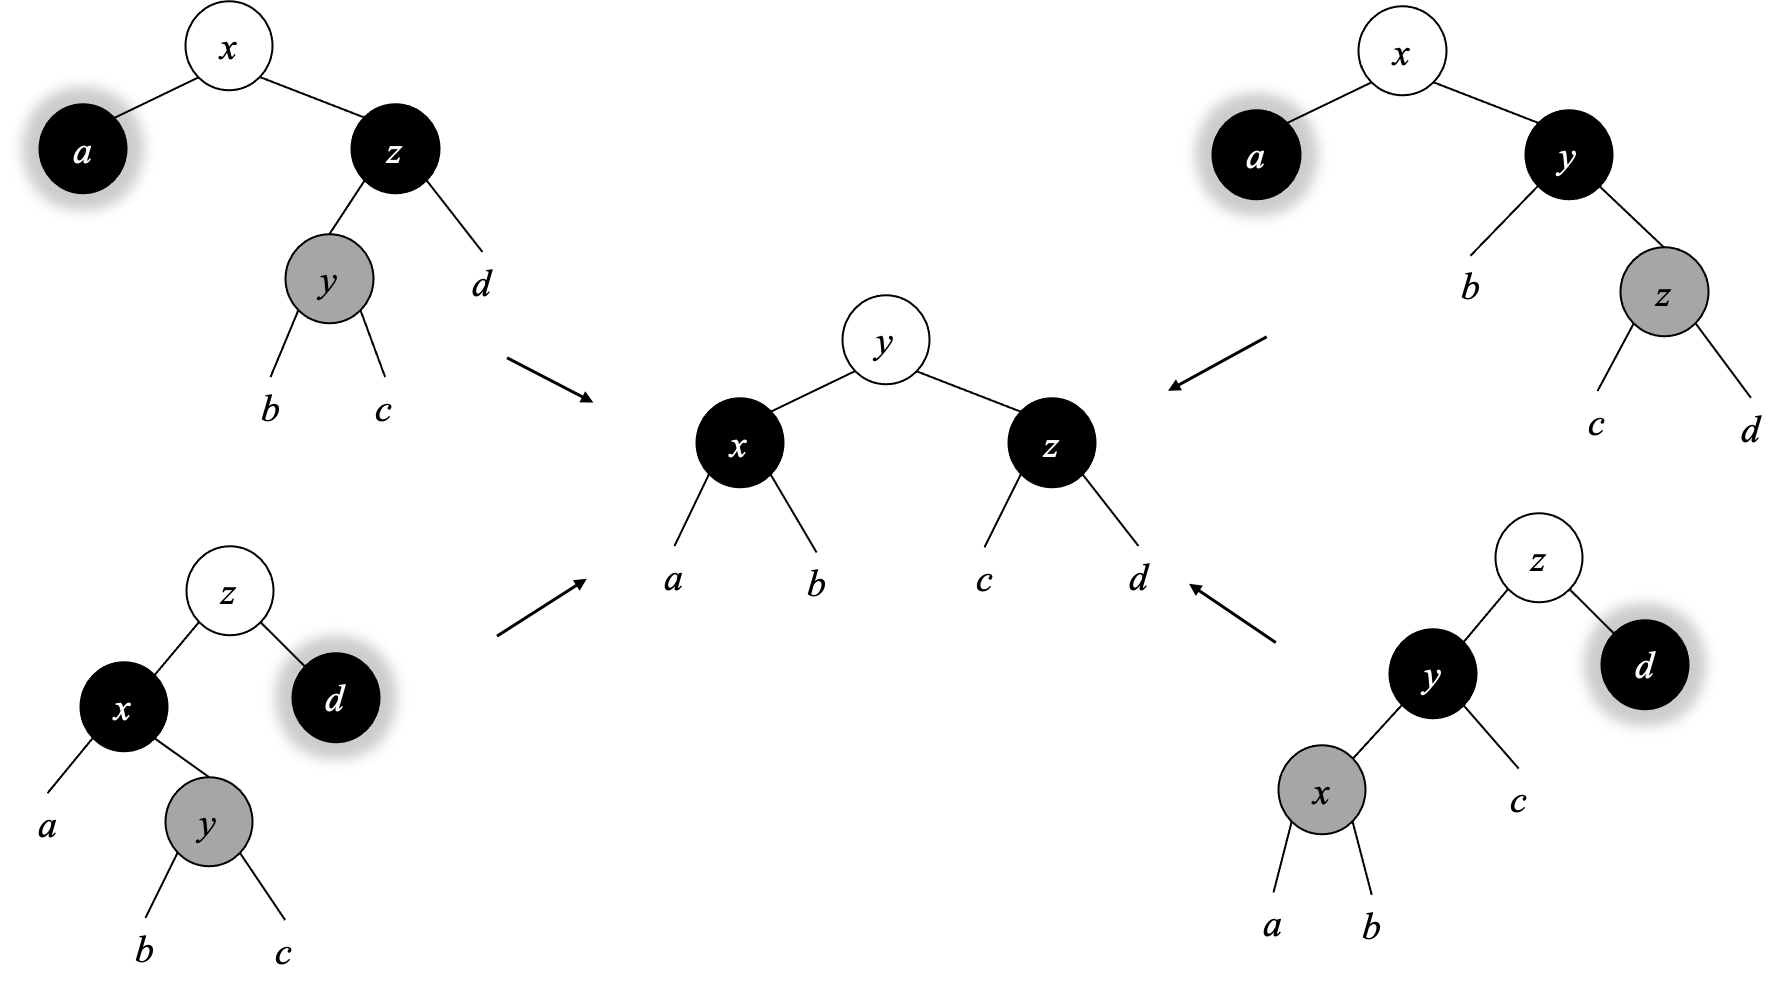
\includegraphics[scale=0.4]{img/del-case1.png}
   \caption{4种子情况可以修复为统一的形式}
   \label{fig:del-case1}
\end{figure}

我们通过模式匹配来处理这四种子情况:

\be
\resizebox{\textwidth}{!}{\ensuremath{
\begin{array}{rcl}
%\text{case 1 up left:} & & \\
fixB^2\ \mathcal{C}\ a_{\mathcal{B}^2}\ x\ (\mathcal{B}, (\mathcal{R}, b, y, c), z, d) & = & (\mathcal{C}, (\mathcal{B}, shiftB(a), x, b), y, (\mathcal{B}, c, z, d)) \\
%\text{case 1 up right:} & & \\
fixB^2\ \mathcal{C}\ a_{\mathcal{B}^2}\ x\ (\mathcal{B}, b, y, (\mathcal{R}, c, z, d)) & = & (\mathcal{C}, (\mathcal{B}, shiftB(a), x, b), y, (\mathcal{B}, c, z, d)) \\
%\text{case 1 bottom left:} & & \\
fixB^2\ \mathcal{C}\ (\mathcal{B}, a, x, (\mathcal{R}, b, y, c))\ z\ d_{\mathcal{B}^2} & = & (\mathcal{C}, (\mathcal{B}, a, x, b), y, (\mathcal{B}, c, z, shiftB(d))) \\
%\text{case 1 bottom right:} & & \\
fixB^2\ \mathcal{C}\ (\mathcal{B}, (\mathcal{R}, a, x, b), y, c)\ z\ d_{\mathcal{B}^2} & = & (\mathcal{C}, (\mathcal{B}, a, x, b), y, (\mathcal{B}, c, z, shiftB(d))) \\
\end{array}
}}
\label{eq:db-case-1}
\ee

其中$a_{\mathcal{B}^2}$表示节点$a$是双重黑色,可以是分枝节点或$\pmb{\varnothing}$。

\textbf{情况2:双重黑色节点的兄弟节点为红色。}可以通过旋转,将其变换为情况1。如图\ref{fig:del-case2}所示。

\begin{figure}[htbp]
  \centering
  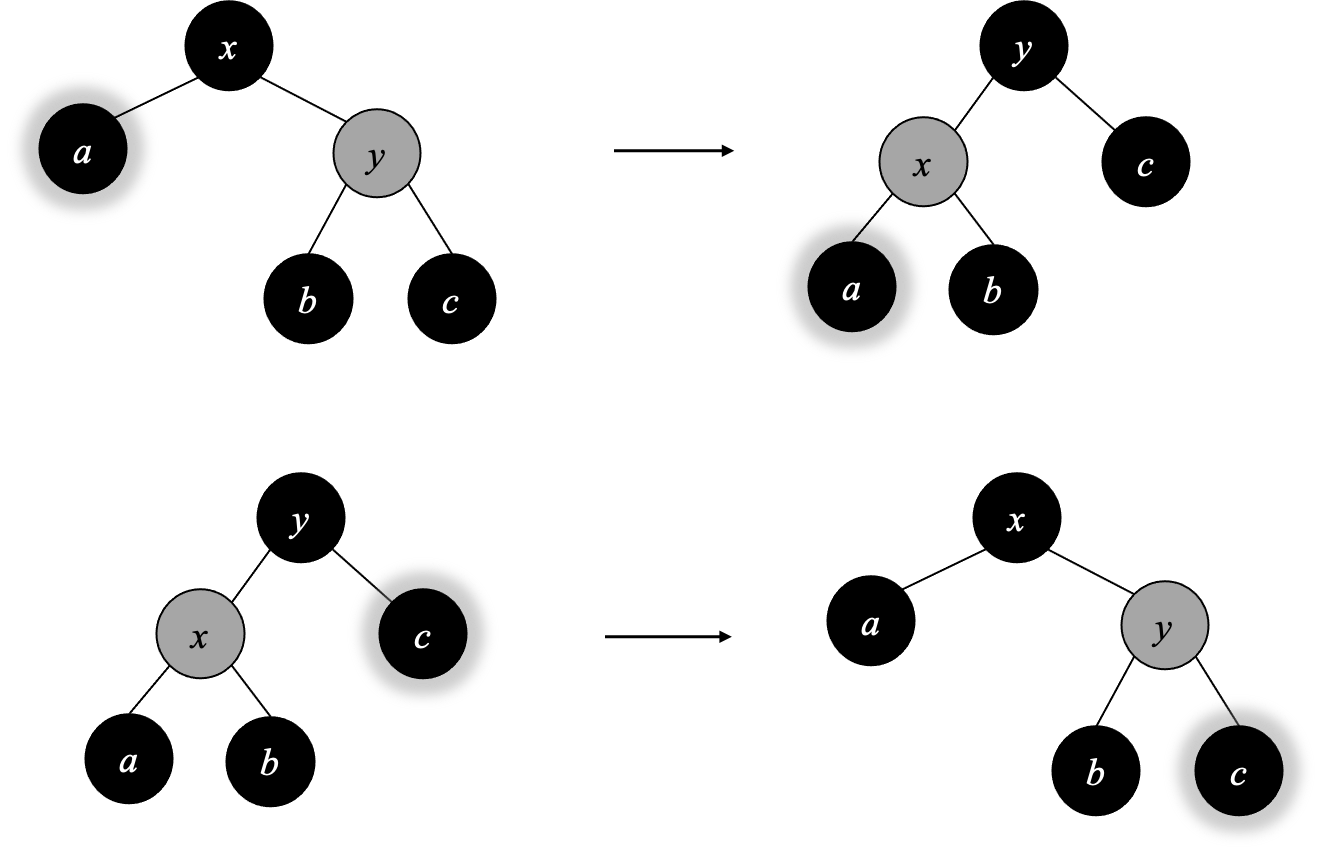
\includegraphics[scale=0.4]{img/del-case2.png}
  \caption{双重黑色节点的兄弟节点为红色}
  \label{fig:del-case2}
\end{figure}

我们在公式(\ref{eq:db-case-1})的基础上增加情况2的修复:

\be
%\resizebox{\textwidth}{!}{\ensuremath{
\begin{array}{rcl}
\text{...} & & \\
%\text{case 2 up:} & & \\
fixB^2\ \mathcal{B}\ a_{\mathcal{B}^2}\ x\ (\mathcal{R}, b, y, c) & = & fixB^2\ \mathcal{B}\ (fixB^2\ \mathcal{R}\ a\ x\ b)\ y\ c \\
%\text{case 2 bottom:} & & \\
fixB^2\ \mathcal{B}\ (\mathcal{R}, a, x, b)\ y\ c_{\mathcal{B}^2} & = & fixB^2\ \mathcal{B}\ a\ x\ (fixB^2\ \mathcal{R}\ b\ y\ c)
\end{array}
%}}
\label{eq:db-case-2}
\ee

\textbf{情况3:双重黑色的兄弟节点,该兄弟节点的两个子节点都是黑色。}这种情况下,我们将兄弟节点染成红色,将双重黑色变回黑色,然后将双重黑色属性向上传递一层到父节点。如图\ref{fig:del-case3}所示。

\begin{figure}[htbp]
  \centering
  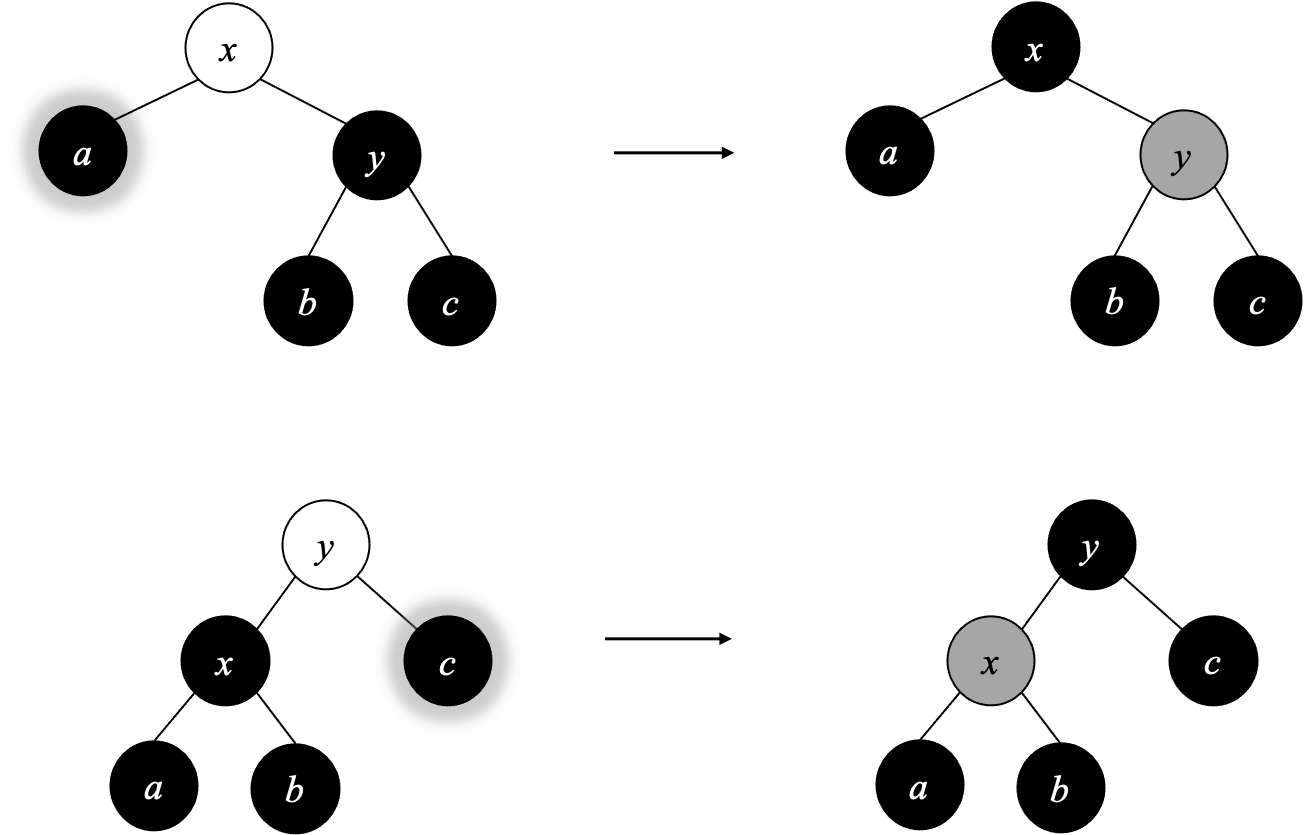
\includegraphics[scale=0.4]{img/del-case3.png}
  \caption{将双重黑色向上传递}
  \label{fig:del-case3}
\end{figure}

有两种对称情况。对于上方的情况,如果$x$是红色,则变为黑色,否则变为双重黑色;对于下方的情况$y$的变化与此类似。我们继续在式(\ref{eq:db-case-2})的基础上增加此种修复:

\be
%\resizebox{\textwidth}{!}{\ensuremath{
\begin{array}{rcl}
\text{...} & & \\

fixB^2\ \mathcal{C}\ a_{\mathcal{B}^2}\ x\ (\mathcal{B}, b, y, c) & = & shiftB\ (\mathcal{C}, (shiftB\ a), x, (\mathcal{R}, b, y, c)) \\

fixB^2\ \mathcal{C}\ (\mathcal{B}, a, x, b)\ y\ c_{\mathcal{B}^2} & = & fixB^2\ \mathcal{B}\ a\ x\ (fixB^2\ \mathcal{R}\ b\ y\ c) \\

fixB^2\ \mathcal{C}\ l\ k\ r\ & = & (\mathcal{C}, l, k, r) \\
\end{array}
%}}
\label{eq:db-case-3}
\ee


至此,我们对于双重黑色的全部情况都完成了修复。算法被定义为一个递归函数。它有两个终止条件:一个是$p1.1$和$p1.2$,双重黑色节点被直接消除了;另外一个是将双重黑色继续向上传递,直到根节点。由于算法最终会将根节点染成黑色,所以双重黑色也会被消除。

综合公式(\ref{eq:db-case-1a})、(\ref{eq:db-case-2})和(\ref{eq:db-case-3a}),我们可以得到最终的Haskell删除程序。

\begin{lstlisting}[style=Haskell]
-- 兄弟节点为黑色,并且有一个红色子节点
fixDB color a@(Node BB _ _ _) x (Node B (Node R b y c) z d)
      = Node color (Node B (makeBlack a) x b) y (Node B c z d)
fixDB color BBEmpty x (Node B (Node R b y c) z d)
      = Node color (Node B Empty x b) y (Node B c z d)
fixDB color a@(Node BB _ _ _) x (Node B b y (Node R c z d))
      = Node color (Node B (makeBlack a) x b) y (Node B c z d)
fixDB color BBEmpty x (Node B b y (Node R c z d))
      = Node color (Node B Empty x b) y (Node B c z d)
fixDB color (Node B a x (Node R b y c)) z d@(Node BB _ _ _)
      = Node color (Node B a x b) y (Node B c z (makeBlack d))
fixDB color (Node B a x (Node R b y c)) z BBEmpty
      = Node color (Node B a x b) y (Node B c z Empty)
fixDB color (Node B (Node R a x b) y c) z d@(Node BB _ _ _)
      = Node color (Node B a x b) y (Node B c z (makeBlack d))
fixDB color (Node B (Node R a x b) y c) z BBEmpty
      = Node color (Node B a x b) y (Node B c z Empty)
-- 兄弟节点是红色
fixDB B a@(Node BB _ _ _) x (Node R b y c) = fixDB B (fixDB R a x b) y c
fixDB B a@BBEmpty x (Node R b y c) = fixDB B (fixDB R a x b) y c
fixDB B (Node R a x b) y c@(Node BB _ _ _) = fixDB B a x (fixDB R b y c)
fixDB B (Node R a x b) y c@BBEmpty = fixDB B a x (fixDB R b y c)
-- 兄弟节点和它的两个子节点都是黑色,向上传递黑色
fixDB color a@(Node BB _ _ _) x (Node B b y c) = makeBlack (Node color (makeBlack a) x (Node R b y c))
fixDB color BBEmpty x (Node B b y c) = makeBlack (Node color Empty x (Node R b y c))
fixDB color (Node B a x b) y c@(Node BB _ _ _) = makeBlack (Node color (Node R a x b) y (makeBlack c))
fixDB color (Node B a x b) y BBEmpty = makeBlack (Node color (Node R a x b) y Empty)
-- 其他情况
fixDB color l k r = Node color l k r
\end{lstlisting}

对于含有$n$个节点的红黑树,删除算法的复杂度为$O(\lg n)$。

\begin{Exercise}

\begin{itemize}
\item 选用一种编程语言,实现本节提到的“标记――重建”删除算法:也就是先将要删除的节点标记,但不进行真正的删除。当被标记的节点数目超过50\%的时候,用全部未标记的节点重建树。
\item 为什么不需要在$mkBlk$的调用处,显示地再调用$fixBlack^2$?
\end{itemize}

\end{Exercise}

\section{命令式的红黑树算法$\star$}
\index{红黑树!命令式插入}

通过归纳,我们能够简洁地实现红黑树算法。作为对比,我们来看一下传统的命令式方法。

插入算法的基本思想仍然和二叉搜索树相同。此外,算法需要通过树的旋转操作修复平衡。

\begin{algorithmic}[1]
\Function{Insert}{$T, k$}
  \State $root \gets T$
  \State $x \gets$ \Call{Create-Leaf}{$k$}
  \State \Call{Color}{$x$} $\gets$ RED
  \State $p \gets$ NIL
  \While{$T \neq$ NIL}
    \State $p \gets T$
    \If{$k <$ \Call{Key}{$T$}}
      \State $T \gets $ \Call{Left}{$T$}
    \Else
      \State $T \gets $ \Call{Right}{$T$}
    \EndIf
  \EndWhile
  \State \Call{Parent}{$x$} $\gets p$
  \If{$p =$ NIL} \Comment{树$T$为空}
    \State \Return $x$
  \ElsIf{$k <$ \Call{Key}{$p$}}
    \State \Call{Left}{$p$} $\gets x$
  \Else
    \State \Call{Right}{$p$} $\gets x$
  \EndIf
  \State \Return \Call{Insert-Fix}{$root, x$}
\EndFunction
\end{algorithmic}

当插入一个新节点时,我们将其染成红色,然后修复平衡并返回。上述算法可以转换为下面的Python例子程序。

\lstset{language=Python}
\begin{lstlisting}
def rb_insert(t, key):
    root = t
    x = Node(key)
    parent = None
    while(t):
        parent = t
        if(key < t.key):
            t = t.left
        else:
            t = t.right
    if parent is None: #树为空
        root = x
    elif key < parent.key:
        parent.set_left(x)
    else:
        parent.set_right(x)
    return rb_insert_fix(root, x)
\end{lstlisting}

总共有3种基本情况需要修复。如果考虑左右对称,则需要修复6种情况。3种基本情况中的两种可以合并。新插入节点的父节点,以及父节点的兄弟节点均为红色。我们可以把它们变为黑色,然后把新插入节点的祖父节点染为红色。修复算法的实现如下:

\begin{algorithmic}[1]
\Function{Insert-Fix}{$T, x$}
  \While{\Call{Parent}{$x$} $\neq$ NIL $\land$ \textproc{Color}(\Call{Parent}{$x$}) = RED}
    \If{\textproc{Color}(\Call{Uncle}{$x$}) $=$ RED}
      \Comment{情况1:$x$的叔父节点是红色}
      \State \textproc{Color}(\Call{Parent}{$x$}) $\gets$ BLACK
      \State \textproc{Color}(\Call{Grand-Parent}{$x$}) $\gets$ RED
      \State \textproc{Color}(\Call{Uncle}{$x$}) $\gets$ BLACK
      \State $x \gets$ \Call{Grand-Parent}{$x$}
    \Else
      \Comment{$x$的叔父节点是黑色}
      \If{\Call{Parent}{$x$} = \textproc{Left}(\Call{Grand-Parent}{$x$})}
        \If{ $x =$ \textproc{Right}(\Call{Parent}{$x$})}
          \Comment{情况2:$x$是右侧子节点}
          \State $x \gets$ \Call{Parent}{$x$}
          \State $T \gets$ \Call{Left-Rotate}{$T, x$}
        \EndIf
        \Comment{情况3:$x$是左侧子节点}
        \State \textproc{Color}(\Call{Parent}{$x$}) $\gets$ BLACK
        \State \textproc{Color}(\Call{Grand-Parent}{$x$}) $\gets$ RED
        \State $T \gets$ \textproc{Right-Rotate}($T$, \Call{Grand-Parent}{$x$})
      \Else
         \If{ $x =$ \textproc{Left}(\Call{Parent}{$x$})}
          \Comment{情况2的对称情况}
          \State $x \gets$ \Call{Parent}{$x$}
          \State $T \gets$ \Call{Right-Rotate}{$T, x$}
        \EndIf
        \Comment{情况3的对称情况}
        \State \textproc{Color}(\Call{Parent}{$x$}) $\gets$ BLACK
        \State \textproc{Color}(\Call{Grand-Parent}{$x$}) $\gets$ RED
        \State $T \gets$ \textproc{Left-Rotate}($T$, \Call{Grand-Parent}{$x$})
      \EndIf
    \EndIf
  \EndWhile
  \State \Call{Color}{$T$} $\gets$ BLACK
  \State \Return $T$
\EndFunction
\end{algorithmic}

这一算法向红黑树中插入key的复杂度为$O(\lg n)$。和前面定义的$balance$函数相比,我们可以发现它们的差异。两种方法不仅仅在篇幅长短上不同,具体的逻辑也不一样。即使输入同一序列的key,两种方法也会构造出不同的红黑树。并且,和这一命令式算法相比,前面使用模式匹配的函数式算法存在一些性能上的损失。Okasaki在\cite{okasaki}中给出了关于函数式红黑树插入算法性能的详细分析。

上述修复算法可以实现为如下的Python例子程序。

\lstset{language=Python}
\begin{lstlisting}
# 修复连续的红色节点
def rb_insert_fix(t, x):
    while(x.parent and x.parent.color==RED):
        if x.uncle().color == RED:
            # 情况1: ((a:R x:R b) y:B c:R) ==> ((a:R x:B b) y:R c:B)
            set_color([x.parent, x.grandparent(), x.uncle()],
                      [BLACK, RED, BLACK])
            x = x.grandparent()
        else:
            if x.parent == x.grandparent().left:
                if x == x.parent.right:
                    # 情况2: ((a x:R b:R) y:B c) ==> 情况3
                    x = x.parent
                    t=left_rotate(t, x)
                # 情况3: ((a:R x:R b) y:B c) ==> (a:R x:B (b y:R c))
                set_color([x.parent, x.grandparent()], [BLACK, RED])
                t=right_rotate(t, x.grandparent())
            else:
                if x == x.parent.left:
                    # 情况2': (a x:B (b:R y:R c)) ==> 情况3'
                    x = x.parent
                    t = right_rotate(t, x)
                # 情况3': (a x:B (b y:R c:R)) ==> ((a x:R b) y:B c:R)
                set_color([x.parent, x.grandparent()], [BLACK, RED])
                t=left_rotate(t, x.grandparent())
    t.color = BLACK
    return t
\end{lstlisting}

图\ref{fig:imperative-insert}给出了两棵红黑树,它们是使用和图\ref{fig:insert-example}中完全相同的序列构造出的。我们可以发现它们明显不同。

\begin{figure}[htbp]
   \centering
   \subcaptionbox{}{\includegraphics[scale=0.4]{img/clrs-fig-13-4.ps}}
   \subcaptionbox{}{\includegraphics[scale=0.4]{img/python-insert.ps}}
   \caption{命令式算法构建出的红黑树}
   \label{fig:imperative-insert}
\end{figure}

红黑树的命令式删除算法和插入算法相比更为复杂。我们不在正文给出,读者可以参考本书附录B了解其详细实现。

\section{其它}
红黑树是最广泛使用的一种平衡二叉搜索树。另外一种自平衡二叉树是AVL树,我们将在下一章介绍。红黑树可以帮助我们了解其它更复杂的数据结构。如果我们将子节点的数目从两个扩展到$k$个,并且保持树的平衡,就可以演化到B树。如果我们在边上,而非在节点中存储数据,我们就得到了Trie。由于常见红黑树算法需要处理很多情况,代码篇幅较长,初学者往往会感觉红黑树很复杂。

Okasaki的工作使得红黑树算法变得容易理解。这激发了很多其它程序设计语言进行类似的实现\cite{rosetta}。本书中给出的Splay树、AVL树等模式匹配算法也是受到这一启发而完成的。

\ifx\wholebook\relax \else
\begin{thebibliography}{99}

\bibitem{CLRS}
Thomas H. Cormen, Charles E. Leiserson, Ronald L. Rivest and Clifford Stein.
``Introduction to Algorithms, Second Edition''. ISBN:0262032937. The MIT Press. 2001 (《算法导论》中文版)

\bibitem{okasaki}
Chris Okasaki. ``FUNCTIONAL PEARLS Red-Black Trees in a Functional Setting''. J. Functional Programming. 1998

\bibitem{okasaki-blog}
Chris Okasaki. ``Ten Years of Purely Functional Data Structures''. http://okasaki.blogspot.com/2008/02/ten-years-of-purely-functional-data.html

\bibitem{wiki-rbt}
Wikipedia. ``Red-black tree''. http://en.wikipedia.org/wiki/Red-black\_tree

\bibitem{lyn}
Lyn Turbak. ``Red-Black Trees''. http://cs.wellesley.edu/~cs231/fall01/red-black.pdf Nov. 2, 2001.

\bibitem{sgi-stl}
SGI STL. http://www.sgi.com/tech/stl/

\bibitem{rosetta}
Pattern matching. http://rosettacode.org/wiki/Pattern\_matching

\end{thebibliography}

\end{document}
\fi
